\newpage
\section{Analysis}

Once the code has been completed and the functionality has been verified (See section xxx for verification) we have automated the process to run the application for every possible input size $1 \leq size \leq 128$ and collect all the timing information to conduct performance analysis and get more insight into the application's behavior under different input sizes.

Figure~\ref{fig:perf_plot} shows execution time for different valid input sizes for different configurations. To facilitate the analysis a more elaborate plot with speedups has been made in Figure~\ref{fig:speedup_plot} which shows speedups for different valid input sizes for DSP+NEON and NEON only configurations. (Note that the spikes in the plots are due to the fact that the operating system is not real-time) This figure shows us a number of useful insights:

\begin{itemize}
\item{NEON+DSP shows slowdown for $size < 60 + \epsilon$}
\item{NEON only configuration performs better for $size < 90 + \epsilon$}
\item{NEON+DSP configuration is best for $size >90 + \epsilon$}
\item{NEON only configuration performs better than serial execution $ \forall size$}

\end{itemize}



\begin{figure}[h!]
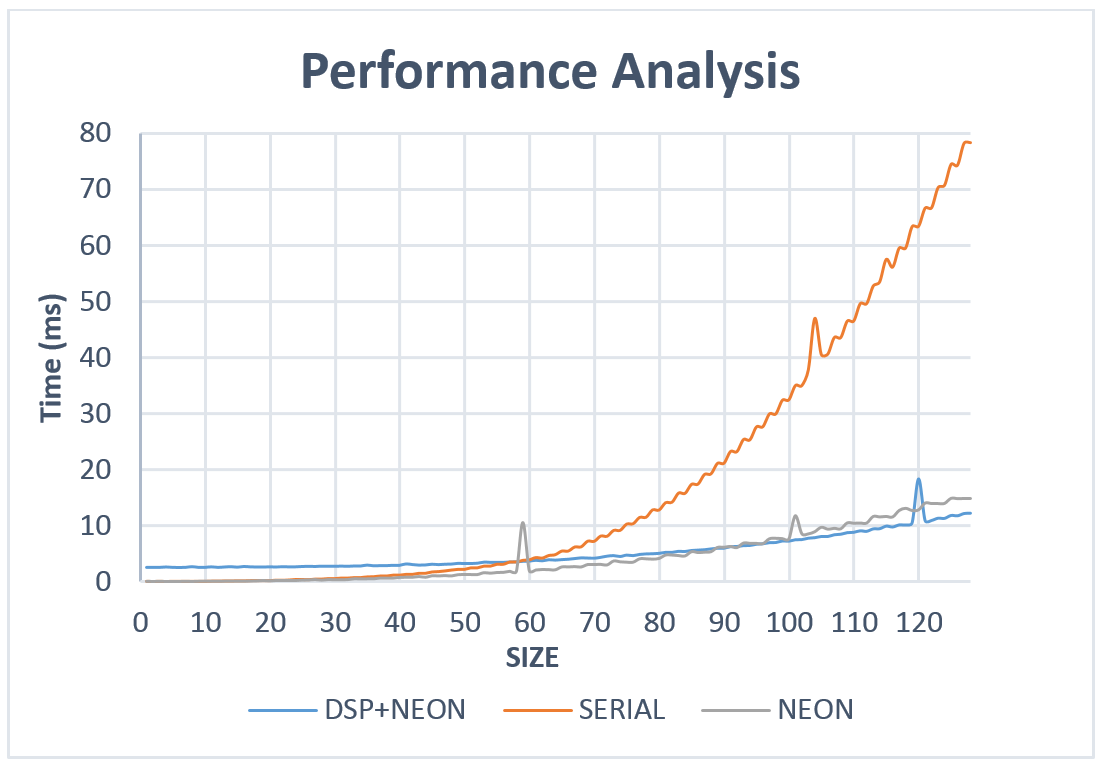
\includegraphics[width=\textwidth]{analysis/perf_plot}
\caption{Performance Analysis plot: Execution times as a function of input size for different configurations}
\label{fig:perf_plot}
\end{figure}


\begin{figure}[h!]
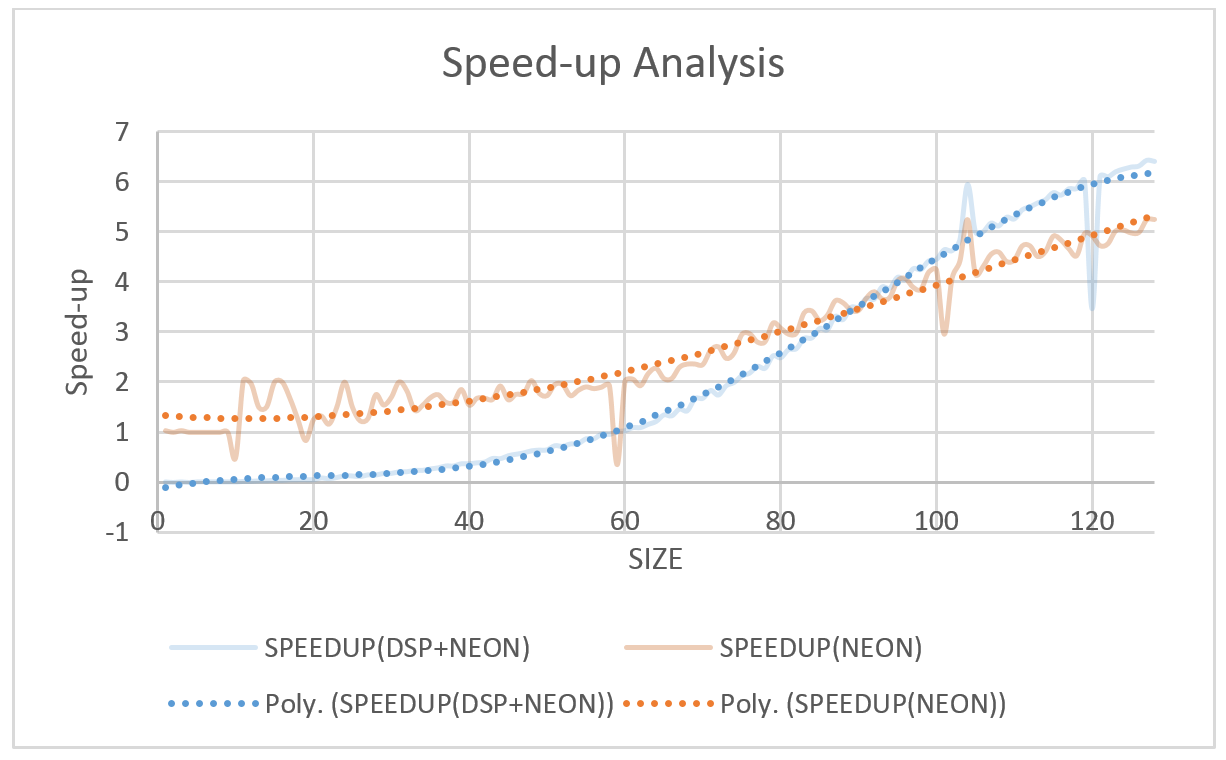
\includegraphics[width=\textwidth]{analysis/speedup_plot}
\caption{Speed-up plot: Achievable speed-up as a function of input size for different configurations}
\label{fig:speedup_plot}
\end{figure}

\subsection{Theoretical Upper Bound on the Speed-Up}

we are using the beagle-board to speed-up our reference application( Multiplications). Our plan is to distribute the  computation load on both the neon and Dsp equally. As DSP has two cores which can perform two operation simultaneously. This means on the DSP we can perform four operations at same time. And similarly by using Neon we can also perform four operations at a time. 
In order to simplify the calculation for upper bound on the speed-up, we  have made following assumptions: 
\begin{itemize}
\item All the operations takes single clock cycle to complete.
\item The time that is consumed in communication between the processors is zero. 
\item The time to load data data into the processors is negligible. 
\end{itemize}

The complexity of Serial multiplications= O(n^3).

In order to make our calculations simple, we have assumed  that n = 16. so our task is to perform the  multiplications of two 16x16 matrices . 

As serial multiplications takes n^3 cycles to complete, so number of cycles required to complete multiplications  for n= 16  would be(16^3) 4096.
As  we are distributing our work load equally on the both DSP and Neon,  then the effective work load for each one would be nxn/2. In our current scenario each of the processor will get 16x16/2 matrices.

As each can perform 4 multiplication operations at a time,so the time , that would require to complete the  all multiplication would be 16x16/8=  32. 

So the fraction  of reference application that is strictly serial for our platform: 32/4096 = 0.0078125

According to Amdahl's law the speed up would be:

S(n) = 1/ (B +( 1- B)/n) 

No of processor are 8, as we can perform 8 calculations at the same time. 

S(8) = 1/(0.0078125 + ( 1 - 0.0078125)/8) = 1 / 0.1318 = 7.6 times . 

 
